\label{ch:lit}

\section{Delayed Heating}

% Most of this comes from 8-/

% Research Reactor accident conditions - LOCA/LOFA : using the ANSI/ANS standard.
The state of the reactor core during an accident is the main focus of research reactor safety analyses.
Accordingly, numerous studies have targeted diverse accident conditions affecting research reactors, such as the \gls*{LOCA} and the \gls*{LOFA}.
% For example, Bajs et al. \cite{bajs_loca_2003} conducted numerical simulations of a LOCA in the IRIS Reactor.
Bajs et al. \cite{bajs_loca_2003} studied the performance of the emergency systems of the \gls* {IRIS} reactor during a LOCA concluding that the reactor core remains at safe temperatures and covered at all times during the event.
Kazeminejad et al. \cite{kazeminejad_thermal_2008} investigated the peak fuel and cladding temperatures of a 10-MW \gls*{IAEA} research reactor after a LOFA with flow inversion.
Hainoun et al. \cite{hainoun_international_2014} introduced a benchmark exercise for thermal-hydraulic solvers to study the LOFA in the IEA-R1 research reactor, where the metrics of interest were the coolant and cladding temperatures, reactor power, and flow rates of different positions in the core.
% And Abdelmaksoud et al. \cite{abdelmaksoud_analysis_2022} examined the passive heat removal by natural convection and radiation of a typical research reactor after a LOCA.
Abdelmaksoud et al. \cite{abdelmaksoud_analysis_2022} examined the possibility of passively cooling by natural convection and radiation the reactor core of a typical research reactor that is completely uncovered after a LOCA.
% % Other applications:
% Other studies targeted the design of nuclear facilities, such as spent fuel storage pools, spent fuel transportation systems, reprocessing plants, and final storage plants, to ensure their safeguards goal \cite{yamamoto_validation_2016}\cite{mozin_delayed_2011}.
% For example, dry storage facilities require the evaluation of the gamma radiation originating in the fuel \cite{gauld_applications_2006}.
% Localized heat deposition
All these studies rely on different versions of the ANSI/ANS standard \cite{ans_decay_1994} for estimating the decay heat after shutdown, assuming that most of the energy from radioactive decay is deposited locally in the region of interest: the reactor core.

Additionally, many software packages, such as Serpent \cite{giot_decay_2018} and ORIGEN \cite{scale}, estimate the decay heat by assuming the local deposition of heat, and diverse studies relied on the same assumption.
Lee et al. \cite{lee_decay_2010} used ORIGEN-2 to compare the decay heat in a \gls*{HTGR} core containing transuranic and uranium fuel.
Ilas et al. \cite{ilas_modeling_2015} calculated the decay heat in the HFIR irradiated fuel using ORIGEN-2.2.
% Some of their results revealed that their calculations yielded a decay heat 46\% larger than the ANSI/ANS standard.
% hawkes_sensitivity_2015 - I am not sure how the gamma heating is calculated, are gammas transported or just come from ORIGEN ? I think they just come from ORIGEN.
Hawkes et al. \cite{hawkes_sensitivity_2015} evaluated with ORIGEN-2.2 the thermal behavior of the AGR-2 experiment in the ATR, an experiment fueled with \gls*{TRISO} particles.
% The experiment heat rate was calculated with MCNP and JMOCUP \cite{sterbentz_mocup_2009}, featuring a couple utility program of MCNP5 and ORIGEN2.2.
% Need for precise method
However, an accurate assessment of the deposited energy across the reactor geometry can better determine the heat removal requirements and ensures an effective cool down.
Moreover, the regulatory authorities and the industry are interested in more precise calculations for economic reasons and \gls*{UQ}.
Therefore, instead of assuming the local deposition of heat, this work focuses on more detailed methods targeting the specific reactor regions hosting the experiments.

The main contributions to the nuclear heating in an operating reactor can be summarized as follows \cite{lemaire_estimation_2015}:
% Table \ref{tab:energy_fission} displays the different components of the energy released through fission.
% As this study places its focus on non-fueled regions of the reactor, the particles of interest are the ones that deposit their energy globally.
% These particles must be transported and heat is deposited during their trajectories.
% % Prompt (including capture gammas) and delayed gammas (from fission product decay) deposit their energy globally and must be transported as well.
% % Need to talk about the heat deposited by charged particles and the necessity of running a gamma-transport simulation.
% \begin{table}[htbp!]
%   \caption{Components of the energy released through fission \cite{brown_monte_2008}.}
%   \label{tab:energy_fission}
%   \begin{tabular}{llll}
%     Quantity                               & Notation        & Deposition site & Value(MeV)  \\
%     Kinetic energy of the fragments        &  Q$_f$          &  Local          & 169.12  \\
%     Kinetic energy of the prompt neutrons  &  Q$_{n,p}$      &  Global         & 4.79  \\
%     Kinetic energy of the delayed neutrons &  Q$_{n,d}$      &  Global         & 7.40E-03  \\
%     Kinetic energy of the prompt gammas    &  Q$_{\gamma,p}$ &  Global         & 6.97  \\
%     Kinetic energy of the delayed gammas   &  Q$_{\gamma,d}$ &  Global         & 6.33  \\
%     Total energy released by delayed betas &  Q$_{\beta}$    &  Local          & 6.50  \\
%     Energy carried away by the neutrinos   &  Q$_\nu$        & -               & 8.75  \\
%     Total energy release per fission (sum) &  Q              &                 & 202.47  \\
%     % Total energy less neutrino energy      &          &                 & 193.72
%     \end{tabular}
% \end{table}
\begin{itemize}
  \item Prompt neutron heating: deposition of the recoil energy of nuclei after a neutron collision and energy deposition of resulting charged particles from neutron interactions - e.g., heating caused by protons released in $(n,p)$ interactions.
  \item Delayed neutron heating: energy deposition of resulting charged particles created with a delay after a neutron interaction - e.g., heating caused by alpha particles resulting from actinide activation and heating caused by beta particles emitted from fission product decay.
  \item Prompt gamma heating: energy deposition of resulting charged particles of photo-atomic and photo-nuclear interactions. Prompt photons are emitted immediately after a neutron interaction. This includes prompt gamma radiation from the rapid de-excitation of the fission fragments and capture gammas.
  \item Delayed gamma heating: same energy deposition mechanism as prompt photons. Delayed photons are the result of activation and fission product decay.
\end{itemize}
% The delayed neutron contribution can be neglected as it is very low and decays within minutes.
% https://nuclear-power.com/wp-content/uploads/2015/10/Yield-of-Delayed-Neutrons.png
% U235 lambda_i [1/sec]: 1) 0.0124, 2) 0.0305, 3) 0.111, 4) 0.301, 5) 1.14, 6) 3.01
% T1/2_i [sec]: 1) 55.89 s ... it is the largest
% % I could include here the calculation of the prompt gammas
% % All contributions / prompt gamma contributions
% Several studies:
% - heating calculations including the prompt neutron, delayed neutron, and prompt gamma contributions
% - focus on determining the ratio between delayed and prompt gammas.
% % Prompt + delayed gamma
% Several studies \cite{lee_gamma_2001} \cite{amharrak_state_2014} \cite{fourmentel_delayed_2015} calculated the gamma heating during reactor operation, which includes both prompt and delayed components.
% % lee_gamma_2001: TRIPOLI-4 + DARWIN, only fission product decay-gammas
% % fourmentel_delayed_2015: TRIPOLI-4, only fission product decay-gammas ??
% % amharrak_state_2014: TRIPOLI-4 + PEPIN-2
% % ambrozic_JSIR2S_2020
% Ambrozic and Snoj \cite{ambrozic_JSIR2S_2020} compared JSIR2S calculations with experimental measurements to validate the code.
% % gruel_heating_2020
% Gruel et al. \cite{gruel_heating_2020} used JSIR2S to calculate the gamma field in the JSI TRIGA Reactor, including both prompt and delayed sources.
% JSIR2S is a code coupling MCNP and Fispact-II \cite{sublet_fispact_2017}.
% While MCNP is responsible for the transport of particles, Fispact-II handles the isotopic inventory and produces the source description for selected particles.
% Shutdown
After reactor shutdown, the prompt emissions no longer contribute to the heating, and we are left with only the delayed neutron and delayed gamma contributions.
% Local vs global
These contributions can be further classified by the location in which the emitted particles deposit their energy.
The delayed neutron heating is caused by charged particles that deposit their energy locally due to their short range.
The delayed gamma heating is caused by photons that deposit their energy globally and must be transported \cite{peterson-droogh_current_2018}.
The following formula calculates the nuclear heating after reactor shutdown or delayed heating
\begin{align}
H_{T} = H_{ch} + H_{\gamma, Tr} \label{eq:heat}
\end{align}
where $H_{T}$ is the total heat deposited in the region of interest, $H_{ch}$ is the energy deposited by charged particles in the region of interest, $H_{\gamma, Tr}$ is the energy deposited in the region of interest resulting from photon transport.

A common method for the calculation of the delayed gamma contribution is the so-called Rigorous 2-Step (R2S) process \cite{chen_rigorous_2002}.
Because the R2S process consists of three steps, this work refers to it as the \textit{formal 3-step process}.
This method consists of the following three steps:
\begin{itemize}
  \item First, a neutron-transport calculation determines the neutron flux spatial and energy distribution during reactor operation.
  \item Second, an activation calculation estimates the energy distribution and emission probability of the photon decay after reactor shutdown.
  \item Third, a photon-transport calculation evaluates the delayed gamma heating.
\end{itemize}

% Nuclear heating in experiment positions - Pre-defined values
Earlier versions of this method accounted for the delayed photons through a fixed-source calculation based on pre-defined gamma emission probabilities.
% ambrosek_improved_1995 - they also calculated the neutron and prompt photon heating
For example, Ambrosek et al. \cite{ambrosek_improved_1995} used this method to calculate the delayed gamma heating component in two ATR experiment positions.
% lee_tripoli_2013
Lee et al. \cite{lee_tripoli_2013} also used this method to calculate the gamma-radiation dose of multiple \gls*{PWR} spent fuel elements.

% Nuclear heating in experiment positions: formal 3-step process
% mozin_delayed_2011
% Mozin \cite{mozin_delayed_2011} implemented the formal 3-step process utilizing MCNP \cite{mcnp} and CINDER to assay the delayed gamma radiation of spent \gls*{LWR} fuel.
% Additionally, they investigated the delayed gamma spectra sensitivity to the actinide content of the fuel.
% Their method actually comprised of four steps, in which the processing of the gamma source was an independent step.
For the formal 3-step process, Mozin \cite{mozin_delayed_2011} utilized MCNP \cite{mcnp} and CINDER \cite{mcnp-cinder} to investigate the delayed gamma spectra sensitivity to the actinide content of spent \gls*{LWR} fuel.
% lemaire_estimation_2015
Lemaire et al. \cite{lemaire_estimation_2015} utilized TRIPOLI-4 \cite{tripoli4} and the point-depletion tool PEPIN-2 \cite{pepin2} to study the delayed gamma contribution from fission product decay in the Jules Horowitz Reactor.
% Lemaire et al. \cite{lemaire_estimation_2015} studied the nuclear heating from prompt neutron, prompt photon, and delayed photons in the Jules Horowitz Reactor.
% Their delayed photon calculation utilized TRIPOLI-4 \cite{tripoli4} and the point-depletion tool PEPIN-2 \cite{pepin2}.
% Their method only accounted for the delayed photons from fission product decay and not the activation product decay.
% noh_estimation_2018 - MCNP6 & ORIGEN-2.1
% Noh et al. \cite{noh_estimation_2018} studied the delayed gamma heating by radiation originated in the activated structures of the High flux Advanced Neutron Application ReactOr (HANARO), a 30-MW research reactor of the \gls*{KAERI}.
% Their implementation coupled MCNP6 and ORIGEN-2.1.
% They calculated the nuclear heating after approximately 8 years of reactor operation in an iridium sample located in multiple irradiation positions - i.e. inner core, outer core, and heavy water reflector tank.
% The calculations considered as radiation sources the structural materials near the irradiation capsule, including the fuel assembly flow tubes, the inner shell separating the reflector tank from the core, and the heavy water reflector tank.
Noh et al. \cite{noh_estimation_2018} coupled MCNP and ORIGEN to study the delayed gamma heating by radiation originated in the activated structures of the High flux Advanced Neutron Application ReactOr (HANARO), a 30-MW research reactor of the \gls*{KAERI}.
% peterson-droogh_current_2018
% Peterson-Droogh and Howard \cite{peterson-droogh_current_2018} summarized in a paper the modeling techniques for the production of iridium-192 in the \gls*{HFIR} at the \gls*{ORNL}.
% The paper described modeling techniques used for the calculation of the heating rates and the activity of the iridium targets.
% The calculation of these metrics are required by thermal-hydraulic calculations and post-irradiation handling.
% Additionally, detailed calculations help in the optimization process of the target design.
% They calculated the prompt neutron and gamma components as well as the delayed components.
% Their calculation scheme of the delayed components can be separated into two.
% The first method relied on the \textit{PIKMT} method, better detailed later in this chapter, for obtaining the delayed gamma contribution from fission product decay.
% The second method used the formal 3-step process for calculating the delayed gamma contribution from activation product decay.
% Their implementation utilized a coupling of MCNP and ORIGEN.
% They utilized ORIGEN, as well, for calculating the heat deposition of charged particles in the iridium targets.
% % The contribution of the prompt photons, delayed photons, and the charged particles from activation product decay are 54\%, 19\%, and 27\% of the total heating rate, respectively.
% % The contribution of the prompt and delayed neutron is negligible.
Peterson-Droogh and Howard \cite{peterson-droogh_current_2018} summarized the modeling techniques for the calculation of the heating rates and the activity of iridium-192 targets in the \gls*{HFIR} at the \gls*{ORNL}.
Their delayed heating calculation was separated into two methods.
The first method was the PIKMT method, described later in this chapter, for obtaining the delayed gamma contribution from fission product decay.
The second method calculated the delayed gamma contribution from activation product decay by coupling MCNP and ORIGEN.

% Other applications of the formal 3-step process
The dose rate evaluation of fusion reactor components is another common application of the formal 3-step process.
% chen_rigorous_2002
Chen et al. \cite{chen_rigorous_2002} calculated the shutdown dose rate of the \gls*{ITER} mid-plane maintenance port coupling MCNP and the FISPACT inventory code \cite{forrest_fispact_1998}.
Other studies using this method include \cite{serikov_advanced_2002, sauvan_development_2016}.
% sauvan_development_2016: R2SUNED = MCNP + ACAB

% Different methods: Direct 1-step process
Valenza et al. \cite{valenza_proposal_2001} introduced another method widely used for shutdown dose rate calculations in fusion reactors.
The method replaces the prompt gamma spectrum with a decay gamma spectrum, and it is better known as the Direct 1-step (D1S) method.
The method requires modifying the nuclear data library so that the delayed gamma radiation replaces the prompt gamma radiation.
For example, the delayed gamma rays from Co-60 replace the prompt gamma rays that accompany the Co-59 $(n, \gamma)$ reaction.
Additionally, the method relies on a depletion solver to account for the build-up and the decay of the considered radionuclides.
Other fusion reactor studies \cite{petrizzi_improvement_2001, palermo_shutdown_2017} used this same method.
% cited by noh_estimation_2008
For fission reactors, Lee et al. \cite{lee_analysis_2008} used this method to calculate the delayed gamma contribution in the HANARO reactor.
% Drawbacks
Although the D1S method is simple once the nuclear data is modified, it is most reliable when the generated radionuclides have short half-lives \cite{noh_estimation_2018}.

% Different methods: PIKMT method
The \textit{PIKMT} method has become predominant in the past few years for delayed gamma heating calculations.
It was first introduced by Brown et al. \cite{brown_monte_2008} and relies on the assumption that the prompt and delayed gamma spectra are similar.
The method uses one neutron-photon coupled simulation using the MCNP PIKMT card to evaluate the energy deposited by prompt gamma radiation originated at fuel fission events, and then it scales it to the delayed gamma component.
% brown_monte_2008
\begin{align}
H_{\gamma, d} &= Q_{\gamma, d} / Q_{\gamma, p} \times F6\!:\!p_{PIKMT}
\end{align}
where $H_{\gamma, d}$ is the delayed gamma heating from the fission product decay, $Q_{\gamma, p}$ and $Q_{\gamma, d}$ is the energy released from fission carried away by the prompt and delayed gamma components, and $F6\!:\!p_{PIKMT}$ is the MCNP $F6$ tally with the PIKMT card.

% PIKMT examples
% Ilas et al. \cite{ilas_impact_2013} used the PIKMT method for studying the conversion of the HFIR's core from \gls*{HEU} to \gls*{LEU}.
% The focus of the study was the neutronic poison buildup and heating rates in the reflector.
% The nuclear heating calculation consisted of two simulations: one for obtaining the neutron and prompt gamma components and the other for the delayed gamma component.
% They compared some of the results obtained with the PIKMT method against previous results obtained with the formal 3-step process for an HFIR reflector redesign study \cite{chang_high_1995}.
% The study concluded that the overall agreement between methods is excellent.
Ilas et al. \cite{ilas_impact_2013} used the PIKMT method for calculating the heating rates in the \gls*{HFIR}’s reflector during a \gls*{HEU} to \gls*{LEU} conversion study.
%
% Davidson et al. \cite{davidson_heat_2017} assessed the feasibility of converting HFIR's fuel from HEU to LEU as well.
% They utilized the PIKMT method for calculating the delayed gamma heating rates in different regions of the reactor.
Davidson et al. \cite{davidson_heat_2017} calculated the delayed gamma heating in different reactor regions using the PIKMT method for another HEU-to-LEU conversion study in HFIR.
% jurbandam_calculation_2018
Jurbandam \cite{jurbandam_calculation_2018} calculated the spatial heat distribution in the SAFARI-1 nuclear reactor, relying on the PIKMT method to account for the delayed gamma contributions.

% Different methods: conclusion
One of the main advantages of the PIKMT method over the formal 3-step process is that it requires only one coupled neutron/photon-transport simulation for obtaining the delayed gamma contribution.
However, it only accounts for the gamma radiation emitted from fission product decay.
In general, when the component of interest is located close to the fuel, the photons from fission product decay become the major contributor to the delayed heating \cite{lemaire_estimation_2015}.
% Actually lemaire says that the activation product contribution is smaller than 2%
In other cases, the photons from activation product decay may have higher contributions.
For those cases, only the formal 3-step process is applicable.
Additionally, the formal 3-step process obtains the charged particle contribution, which is a contribution neglected by the PIKMT method.
Furthermore, the PIKMT method obtains the delayed gamma contribution during reactor operation or immediately after shutdown.
Given that this work is concerned with the time evolution of the delayed heating, the only applicable method here is the formal 3-step process.

% \section{Safety analyis in Research reactors}
% Not sure where/if to place this
% The calculations refer to a document that I couldn't find
% Khericha and Pedersen \cite{khericha_experiment_2003} studied the integrity of an irradiated MOX capsule during a canal draining event.
% The study reveals that a minimum cooling time of 4 hours after reactor shutdown should be established for fueled experiments to assure that melting does not occur.


\section{Transport/Depletion Solvers Background}

% Most of this comes from 6-/

% Need to link the first section to this section
The first two steps in the formal 3-step process are accomplished by coupling a transport and a depletion solver.
This strategy determines the evolution of the material composition in the reactor during operation.
Depletion solvers ignore the geometry of the system, which underscores the need for a transport solver.
The transport solver generates geometry- and material-dependent parameters that the depletion solver relies on.
The depletion solver then calculates the material compositions and returns this information to the transport solver, and a cyclical transfer of information occurs, as shown in Figure \ref{fig:trans-dep}.
% After reactor shutdown, he material composition and the isotopes decay chain provide enough information to determine the energy distribution and emission probability of the photon decay.

\begin{figure}[htbp!]
  \begin{center}
    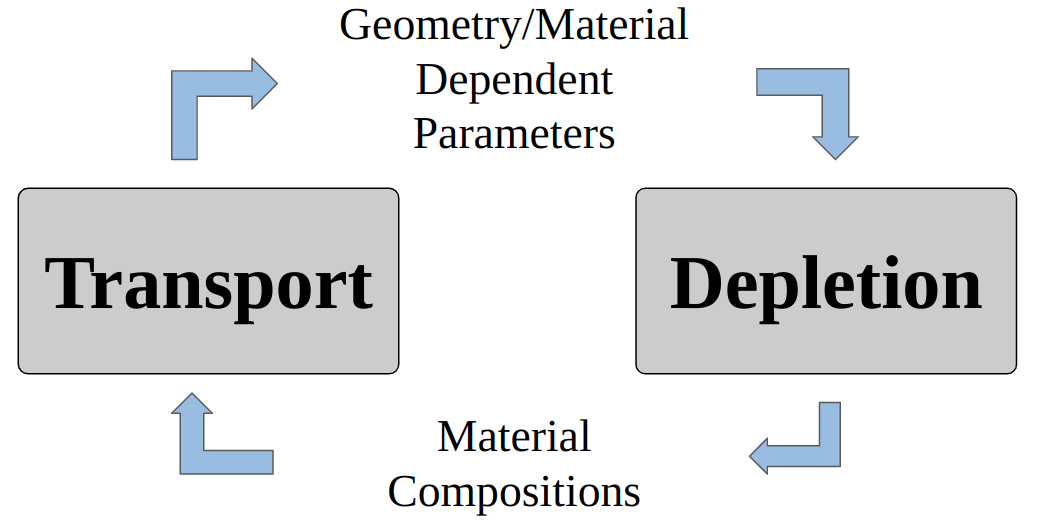
\includegraphics[scale=0.3]{figures/diagram_1}
  \end{center}
  \caption{Typical workflow of a transport/depletion solver.}
  \label{fig:trans-dep}
\end{figure}

There are several software packages available with these capabilities.
Table \ref{tab:background} summarizes some popular transport/depletion software packages that have been developed over the past 25 years.
This list is not meant to be extensive and instead provides the reader with an overview of past developments.
The motivation for the development of these tools varies.
Some were created to address specific projects, such as MOCUP \cite{mocup}, which was developed to simulate isotope depletion of the \gls*{ATR} and the Advanced Neutron Source, and Monteburns \cite{monte}, which was created to simulate isotope depletion for the Accelerator Transmutation of Waste (ATW) project at the \gls*{LANL}.

Additionally, MCNP’s lack of depletion capabilities motivated the development of many of these software packages, as well as the addition of depletion subroutines to MCNP itself \cite{mcnp-cinder}.
The integration of CINDER90 into MCNP provides a self-contained Monte Carlo/depletion capability in a single tool.
Serpent \cite{leppanen_serpent_2015} is another example of a Monte Carlo solver with self-contained depletion subroutines.

% MAYBE: add MCNP versions
\begin{table}[htbp!] %htbp! or H
  \centering
  \caption{List of previous Transport/Depletion software packages.}
  \label{tab:background}
  \begin{tabular}{ccccc}
    \toprule
    Tool       & Reference    & Transport  & Depletion  & Year developed \\
    \midrule
    MOCUP      & \cite{mocup} & MCNP       & ORIGEN2    & 1995 \\ %MCNP4A
    Monteburns & \cite{monte} & MCNP       & ORIGEN2    & 1998 \\ %MCNP4B
    MCODE-2.2  & \cite{mcode} & MCNP       & ORIGEN2    & 2008 \\ %MCNP4C
    VESTA      & \cite{vesta} & MCNP       & ORIGEN2/Phoenix & 2008 \\ %MCNP (any version)
    MCNP       & \cite{mcnp}  & \multicolumn{2}{c}{MCNP (CINDER90)} & 2009 \\ 
    Serpent    & \cite{leppanen_serpent_2015} & \multicolumn{2}{c}{Serpent (CRAM)} & 2010 \\
    \bottomrule
  \end{tabular}
\end{table}

Most of these tools, however, still rely on ORIGEN2, which was deprecated and lost support more than three decades ago.
The current version is ORIGEN/SCALE (sometimes called ORIGEN-S or just ORIGEN), which uses the \gls*{CRAM} \cite{cram} to solve the system of depletion equations.
While the open literature describes various depletion algorithms, the three most relevant are CINDER90 \cite{mcnp-cinder}, MATREX \cite{scale}, and \gls*{CRAM}.
MCNP uses CINDER90, ORIGEN2 uses MATREX, and ORIGEN uses either MATREX or CRAM.
The accuracy of the CINDER90 algorithm deteriorates for actinide prediction in higher-burnup cases \cite{mcnp-cinder}.
Although increasing CINDER90’s accuracy is possible by using a sub-step method, the CRAM solver produces more accurate solutions even when using longer burnup intervals \cite{vera}.
The MATREX algorithm is a hybrid method combining the Matrix Exponential method and linear chains \cite{origen2}.
While the matrix exponential and linear chains can be solved accurately when independent of each other, accounting for the effects of short and long-lived nuclides in the hybrid method requires additional approximations that lead to a loss of accuracy \cite{origen-cram}.
Overall, CRAM is orders of magnitude more accurate than other depletion algorithms currently available \cite{vera, origen2, origen-cram}.
Furthermore, in most cases, the solver is up to several times faster due to not having sub-stepping requirements \cite{origen-cram}.

% Motivation: ATR and active maintenance
As mentioned in Chapter \ref{ch:intro}, this work intends to demonstrate the modeling capabilities of ATR.
The physical configuration of ATR, shown in Figure \ref{fig:atr-view}, gives the reactor the unique capability to operate simultaneously at different power levels in the corner lobes.
This feature enables independent testing conditions within the same operating cycle for experiments located in different reactor regions \cite{atr}.

\begin{figure}[htbp!]  % or H
  \begin{center}
    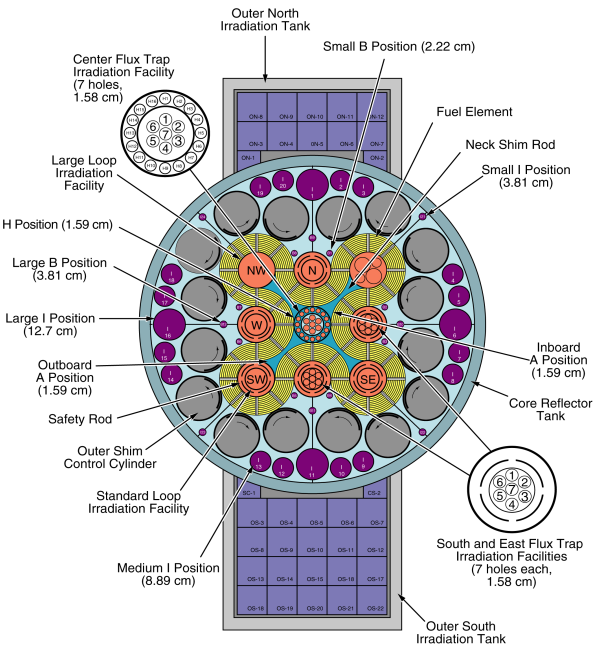
\includegraphics[scale=0.45]{figures/atr_view}
  \end{center}
  \caption{ATR cross sectional diagram and irradiation locations. Image reproduced from \cite{atr}.}
  \label{fig:atr-view}
\end{figure}

The analysis of ATR experiments requires the transport/depletion solver to have a lobe power scaling capability to properly calculate the neutron flux normalization factor and hence obtain the right depletion rates.
% A study within the section dedicated to MOAA could be to compare the flux and also depletion rates of an experiment when using and not using <atr>True</atr>.
While multiple tools have targeted ATR in the past, most of them are no longer maintained.
Active maintenance has many desirable features, including the development of new capabilities, bug catching and fixing, code updates for compliance with quality assurance requirements, among others.
% Motivation: computational requirments
% Finally, continuous energy Monte Carlo depletion calculations have high computational requirements, being memory-intensive tasks with long computation times \cite{vesta-2}.
Finally, continuous energy Monte Carlo depletion calculations have high computational requirements with long computation times.

% Conclusions
Overall, a tool relying on ORIGEN (and CRAM) that can model ATR and has low computational requirements can fulfill this thesis' needs.
The tool with all the desired capabilities is MOAA \cite{fairhurst_development_2022}, which is described in detail in Chapter \ref{ch:delayedheat}.


\section{Machine Learning}

% Why is this necessary?
As stated in Chapter \ref{ch:intro}, one of the objectives of this Ph.D. thesis is to accelerate the prediction of the bounding event outcome (capsule melts or does not melt).
This method relies on multiple machine learning algorithms.
This section of the thesis motivates the choice of the algorithms and describes them briefly.

% Intro
Machine learning is the branch of artificial intelligence that allows computer algorithms to derive relationships from data.
This feature allows them to solve complex problems, while at the same time decreasing the calculations' computational expense.
For example, the high computational expense of physics-based calculations makes them unsuitable for various applications, e.g., real-time reactor control.
Even though the \gls*{HPC} capabilities have increased considerably in the past few decades, they are still not sufficient.
In contrast, machine learning models can emulate the behavior of the input/output relationship of the physics-based model in real-time.

% Traditional ML
Traditional machine learning techniques have been applied in the nuclear engineering field to some extent.
% Safety analysis - Classification - SVM/SVR - IEEE Transactions of Nuclear Science
Na et al. \cite{na_detection_2008} applied \gls*{SVM} and \gls*{SVR} to \gls*{NPP} safety analysis.
During an accident, the NPP operators may have insufficient time to analyze the data and swiftly mitigate it.
Their work studied the applicability of \gls*{SVM} and \gls*{SVR} to a \gls*{LOCA} by predicting the break size and its location.
The model used multiple reactor signals, including core exit temperature, pressurizer water level, and containment pressure.

% Regression - SVR - Nuclear Engineering and Technology
NPPs safety systems calculate a number of safety-critical parameters and trip the reactor when they exceed the operating limits.
An accurate estimation of the local power density is necessary for the safe operation of an NPP for preventing the fuel rod from melting.
Bae et al. \cite{bae_estimation_2009} applied \gls*{SVR} to \gls*{NPP} online monitoring.
Their study accurately estimated the local power density based on different signals of the reactor coolant system, including reactor power, core inlet temperature, and coolant flow rate.

% Reactor control - Regression - SVR - Annals of Nuclear Energy
Zeng et al. \cite{zeng_machine_2017} created a machine learning-based system for autonomous control of small reactors.
The system consisted of a prediction module using \gls*{SVR} to estimate the state of some system variables, such as coolant and fuel temperatures, flux, and power history.
The prediction module fed into a decision module, which consisted of the control decision making and control system motion.
They demonstrated the system prediction module for a reactivity insertion event in a 20 MW$_{th}$ \gls*{TFHR}.

% Predictive maintenance - Classification - SVM and Logistic regression - Nuclear Engineering and Technology
Gohel et al. \cite{gohel_predictive_2020} developed a framework utilizing \gls*{SVM} and \gls*{LogR} for conducting predictive maintenance of \glspl*{NPP}.
Predictive maintenance allows operators to mitigate component failures and to increase the power plant availability.
Their framework intended to predict the failure of a power plant infrastructure in future cycles based on sensor real-time data.
Due to the lack of real NPP data, the paper demonstrated the framework by applying it to the degradation of a turbofan engine.

% Several - Nuclear Engineering and Design
Blevins and Yang \cite{blevins_machine_2020} discussed the suitability of machine learning for manufacturing in nuclear engineering.
Their article presented an overview and examples of applications of multiple machine learning techniques, such as \gls*{DTR}, \gls*{RFR}, \gls*{SVM}, \gls*{KNN}, and \glspl*{FNN}, to advanced manufacturing.
As many of these algorithms have not been yet applied to advanced manufacturing in the nuclear engineering field, they extrapolated these methods from different engineering applications, including semiconductor doping, manufacturing defect detection, and additive manufacturing parameter optimization, among others.

% Deep learning
Additionally, deep-learning, which is a sub-field of machine learning, has also been applied to nuclear engineering problems.
Deep-learning algorithms are more complex and abstract than traditional machine learning algorithms.
Nevertheless, a higher level of abstraction allows them to automate some pieces of the training process and, hence, eliminate some of the human intervention.
% Online Monitoring - ANNs - Nuclear Technology
In 1992, Guo and Uhrig \cite{guo_use_1992} presented one of the first applications of \glspl*{ANN} to nuclear engineering.
They developed a model for online monitoring that was able to predict the thermal performance and gross heat rate of the Sequoyah \gls*{NPP}.
The model utilized a hybrid neural network, comprising a clustering stage and an \gls*{FNN}, trained with sensor signals from the plant.
Additionally, they applied a sensitivity analysis to the network to determine the variables that affected the heat rate the most.
This kind of study allows power plant personnel to determine the cause of anomalies and, hence, provide a controlling basis for them.

% Optimization - ANNs - Annals of Nuclear of Nuclear Energy
Erdogan and Melih \cite{erdogan_pwr_2003} developed an optimal loading algorithm for nuclear fuel based on an \gls*{FNN} and a genetic algorithm.
Their algorithm searched for a loading pattern that minimized the initial amount of fuel and satisfied the reactor safety requirements.
Overall, minimizing the use of fuel reduces the operational cost of the plant.
% Optimization - ANNs - Annals of Nuclear Energy
% Fernandes-Faria and Pereira, 2003 \cite{fernandes-faria_nuclear_2003} utilized an \gls{ANN} for minimizing the power peaking factor while maximizing the fuel burnup.
% Control rod position - ANNs - Progress in Nuclear Energy
Andersson et al. \cite{andersson_development_2003} developed an application for online monitoring utilizing \gls*{FNN}.
The network calculated the control rod positions from the axial shape of the neutron flux.
Such an application helps to corroborate the control rod positions during transients.
The neural network could guide that control rod calibration process as well, as the electromechanical position indicators can be recalibrated during operation.
% Online Monitoring - ANNs - Annals of Nuclear Energy
% Souza and Moreira, 2006 \cite{souza_neural_2006} applied ANNs to reactor protection systems.
% Their paper intended to predict in real time the power peak factor based on the control rods position.
% Reactor design ? - ANNs - Annals of Nuclear Energy
Montes et al. \cite{montes_local_2009} applied FNNs to reactor fuel optimization.
The network quickly determined the local power peaking factor in a \gls*{BWR} based on the distribution of fissile and burnable poison materials.
The power peaking factor is a design parameter, and the ability to quickly estimate it reduces the fuel optimization time.
% Time evolution - ANNs - Nuclear Engineering and Design
Gomez Fernandez et al. \cite{gomez_fernandez_nuclear_2017} applied FNNs to reactor accident identification.
Their data comprised multiple sensor signals from a small \gls*{LWR} and the time evolution corresponding to two transient events, a piecewise-constant power ramp and a \gls*{LOFW} accident.
The model was able to accurately identify the transients and predict the time evolution of the reactor.
A model with such features can guide the \gls*{NPP} operators to identify safety issues and to take prompt actions to mitigate the accident.

% CNNs
Other examples of \glspl*{ANN} applied to nuclear engineering include the use of \glspl*{CNN} and \glspl*{RNN}.
For example, Kamuda et al. \cite{kamuda_comparison_2018} applied \glspl*{CNN} to automate isotope identification in gamma-ray spectroscopy.
Wilson \cite{wilson_machine_2019} compared the performance of \gls*{SVR} and a CNN at predicting the reactor power shape for diverse shim blade positions.
Their goal was to demonstrate that machine learning can provide real-time predictions and contribute to the autonomous control of nuclear reactors.

% RNNs
% https://www.analyticsvidhya.com/blog/2022/03/a-brief-overview-of-recurrent-neural-networks-rnn/
% LSTMs
% https://colah.github.io/posts/2015-08-Understanding-LSTMs/
% https://www.analyticsvidhya.com/blog/2021/03/introduction-to-long-short-term-memory-lstm/

% RNNs
\Glspl*{RNN} were created to handle inputs and outputs correlated as part of a sequence.
For example, when predicting the next word of a sentence, the prior words are necessary.
While all inputs and outputs in an FNN are independent of each other, an RNN is a sequential network that allows information to persist and uses it for processing the current input.
In the last few years, \glspl*{RNN} have been successfully applied to various tasks involving sequential inputs, such as speech and language recognition/prediction \cite{mikolov_recurrent_2010}.

% The problem - LSTM - Intro
In practice, RNNs cannot learn long-term dependencies.
When training the network, the back-propagated gradients may grow or shrink significantly at each time step.
Therefore, the gradients may vanish or explode for sufficiently long time series.
This issue is called the vanishing gradient problem, and \glspl*{LSTM} were explicitly designed to avoid it.
LSTMs are a special kind of RNN and are able to learn long-term dependencies.

% LSTM - yang_accident_2018
Yang and Kim \cite{yang_accident_2018} developed a model using LSTMs for accident diagnosis.
The model predicted the evolution of the plant's main variables and identified the accident.
% The trained model demonstrates the feasibility of utilizing LSTM for diagnosing several NPP accidents, including a loss of coolant accident, a steam generator tube rupture, and a main steam line break.
% LSTM - lee_autonomous_2018
Lee et al. \cite{lee_autonomous_2018} created a model using LSTMs for the autonomous operation of safety systems.
% Their model predicted the state of several plant components given multiple physical variables.
% % Given multiple physical variables the predicts the state of several plant components, and hence, reducing the role of human operators in critical decision making.
% % To train a validate their model, they used a compact nuclear simulator featuring a reference PWR.
% LSTM - radaideh_neural-based_2020
Radaideh et al. \cite{radaideh_neural-based_2020} predicted the progression of a \gls*{LOCA} utilizing deep-learning algorithms, including FNNs and LSTMs.
% They utilized two approaches: first, a \gls*{FNN} to fit all outputs in a single model, and second, a \gls{LSTM} network to fit individual models for each output.
% In this approach, the model makes one-step predictions, meaning that it uses the available data for the current time step \textit{t} to predict the following time step \textit{t+1}.
% Then, the actual data at \textit{t+1} is made available so it can be used for making a prediction on the subsequent time step.

% Other examples of LSTM usage outside the nuclear engineering domain include:
% - erosion rate and shoreline evolution forecasting for sandy coasts \cite{calkoen_traditional_2021}
% - speech recognition: Graves, A., & Jaitly, N. (2014). Towards end-to-end speech recognition with recurrent neural networks. International Conference on Machine Learning, 1764–1772.
% - language modeling: Kiros, Salakhutdinov, & Zemel, 2014

% Conclusion
Overall, machine learning has been applied to different areas of nuclear engineering.
The numerous applications described here cover many algorithms that can be classified as traditional machine learning or deep-learning.
This literature survey helps to understand the state of development of this field and can guide the choice of algorithms for this work.
% problem at hand.
However, machine learning has not been yet utilized in applications with similar objectives to this thesis'.
Therefore, Chapter \ref{ch:tf} compares various algorithms performance and analyzes their suitability to this thesis.
